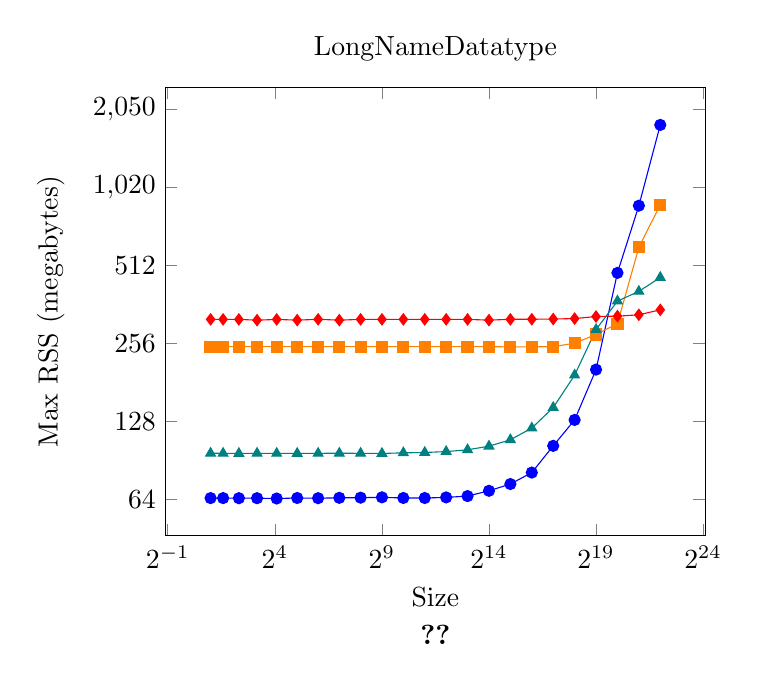
\begin{tikzpicture}
\begin{axis}
[title=LongNameDatatype,
xlabel={Size},
ylabel={Max RSS (megabytes)},
legend to name=legend,
legend columns=2,
xmode=log,
log basis x={2},
ymode=log,
log basis y={2},
yticklabel={
  \pgfkeys{/pgf/fpu=true}
  \pgfmathparse{pow(2,\tick)}
  \pgfmathprintnumber[fixed relative,precision=3]{\pgfmathresult}
  \pgfkeys{/pgf/fpu=false}
}]
\addplot [
color=blue,
mark=o,
only marks,
forget plot
] coordinates {

};
\addplot [
color=orange,
mark=square,
only marks,
forget plot
] coordinates {

};
\addplot [
color=red,
mark=diamond,
only marks,
forget plot
] coordinates {

};
\addplot [
color=teal,
mark=triangle,
only marks,
forget plot
] coordinates {

};
\addplot [
color=blue,
mark=*
] coordinates {
(4194305.0,1787.400192) 
(2097153.0,871.723008) 
(1048577.0,479.604736) 
(524289.0,202.932224) 
(262145.0,129.724416) 
(131073.0,103.010304) 
(65537.0,81.22368) 
(32769.0,73.363456) 
(16385.0,69.070848) 
(8193.0,65.908736) 
(4097.0,65.134592) 
(2049.0,64.786432) 
(1025.0,64.802816) 
(513.0,65.179648) 
(257.0,64.98304) 
(129.0,64.888832) 
(65.0,64.688128) 
(33.0,64.794624) 
(17.0,64.49152) 
(9.0,64.688128) 
(5.0,64.684032) 
(3.0,64.73728) 
(2.0,64.741376) 
};
\addlegendentry{Agda}
\addplot [
color=orange,
mark=square*
] coordinates {
(4194305.0,877.99808) 
(2097153.0,602.324992) 
(1048577.0,305.37728) 
(524289.0,277.209088) 
(262145.0,256.667648) 
(131073.0,248.815616) 
(65537.0,248.549376) 
(32769.0,248.303616) 
(16385.0,248.868864) 
(8193.0,248.868864) 
(4097.0,248.942592) 
(2049.0,248.881152) 
(1025.0,248.958976) 
(513.0,248.815616) 
(257.0,248.950784) 
(129.0,248.950784) 
(65.0,248.7296) 
(33.0,248.946688) 
(17.0,248.889344) 
(9.0,248.840192) 
(5.0,248.860672) 
(3.0,248.705024) 
(2.0,248.782848) 
};
\addlegendentry{Idris 2}
\addplot [
color=red,
mark=diamond*
] coordinates {
(4194305.0,345.239552) 
(2097153.0,330.371072) 
(1048577.0,326.377472) 
(524289.0,325.300224) 
(262145.0,319.496192) 
(131073.0,318.132224) 
(65537.0,317.50144) 
(32769.0,317.353984) 
(16385.0,315.019264) 
(8193.0,317.124608) 
(4097.0,317.181952) 
(2049.0,317.169664) 
(1025.0,317.169664) 
(513.0,317.136896) 
(257.0,317.140992) 
(129.0,314.994688) 
(65.0,317.313024) 
(33.0,315.052032) 
(17.0,316.993536) 
(9.0,314.957824) 
(5.0,317.083648) 
(3.0,317.15328) 
(2.0,317.128704) 
};
\addlegendentry{Lean 4}
\addplot [
color=teal,
mark=triangle*
] coordinates {
(4194305.0,460.292096) 
(2097153.0,406.720512) 
(1048577.0,373.190656) 
(524289.0,289.73056) 
(262145.0,193.159168) 
(131073.0,144.789504) 
(65537.0,120.676352) 
(32769.0,108.740608) 
(16385.0,102.7072) 
(8193.0,99.459072) 
(4097.0,97.886208) 
(2049.0,97.103872) 
(1025.0,96.804864) 
(513.0,96.27648) 
(257.0,96.395264) 
(129.0,96.44032) 
(65.0,96.395264) 
(33.0,96.288768) 
(17.0,96.313344) 
(9.0,96.423936) 
(5.0,96.288768) 
(3.0,96.395264) 
(2.0,96.44032) 
};
\addlegendentry{Rocq}
\end{axis}
\node[anchor=north] at (current axis.below south) {\ref{legend}};
\end{tikzpicture}
